\documentclass[12pt]{report}
\usepackage{geometry}
\usepackage{url,enumerate, amssymb, multirow, anysize, booktabs, threeparttable, amsfonts, bbm}
\usepackage[colorlinks = true,
            linkcolor = blue,
            urlcolor  = blue,
            citecolor = blue,
            anchorcolor = blue]{hyperref}
\usepackage{setspace,listings,dsfont}
%\usepackage{cite}
\usepackage[square,numbers]{natbib}
\bibliographystyle{abbrvnat, lipsum}
\usepackage{mathrsfs, wrapfig}
\usepackage{hanging}
\renewcommand*\thesection{\arabic{section}}
\usepackage{color,soul,amssymb}
\usepackage{fancyhdr, mathtools}
\usepackage{dcolumn, capt-of}
\usepackage{indentfirst, verbatim}
\newcounter{equationset, sectsty, breqn}
\usepackage{setspace,float,lscape,subfigure,amsmath,multirow,color,nag}
\usepackage[font=sf, labelfont={sf,bf}, margin=1cm]{caption}
\captionsetup{font={small,sf,singlespacing}}
\newcommand{\pb}{\mathbb{P}}
\newcommand{\E}{\ensuremath{\mbox{E}}}
% Page style definition
\geometry{margin=1.0in}
\pagestyle{fancy}
% Customize this to your liking.
\setlength{\headheight}{16pt}
\lhead{}\chead{}\rhead{[Simulation] Diffusion Distance}\lfoot{}
\cfoot{\thepage}\rfoot{April, 2016}
\sffamily
\makeatletter
\def\@makechapterhead#1{%
  \vspace*{0\p@}%
  {\parindent \z@ \raggedright \normalfont
    \interlinepenalty\@M
    \Huge\bfseries  \thechapter.\quad #1\par\nobreak
    \vskip 25\p@
  }}
\makeatother


\usepackage{Sweave}
\begin{document}
\Sconcordance{concordance:report2.tex:report2.Rnw:%
1 44 1 1 0 346 1}



\pagenumbering{roman}


\pagenumbering{arabic}

\doublespace


\sffamily
\normalsize
\textit{Most of the works are borrowed from Minh Tang's thesis ``Graph metrics and dimension reduction"}

\section{Network Distance}

 The distance correlation(dCor) $\mathcal{R}^2$ between random vectors $X$($\in \textbf{R}^{p}$) and $Y(\in \textbf{R}^{q})$ is defined based on Euclidean distance between two. In the contexts of network, if node attributes vector $Y$ is all continuous, we can think its distance matrix, but we cannot intuitively think of Euclidean distance for their underlying networks. It is known that a dissimilarity matrix $\Delta$ is a Type-2 Euclidean distance matrix if and only if $\tau(\Delta)$ is positive definite, where $\tau(A) = -\frac{1}{2}(I - 1 1^{T} / n) A (I - 1 1^{T} / n).$ Based on this, we suggest \textit{diffusion distance} as a distance matrix corresponding to Euclidean distance matrix for network. \textit{Diffusion distance} at time $t$ between two nodes can be measured as the dissimilarity of two in the network space with connectivity between them at $t$ step. Let me introduce some notations. 
 
 - Similarity measure $\omega$

$$\omega[i,j] = \mbox{ (the number of synapses starting from i to j)}$$
 

- Transition probability (Assume time homogeneous Markov chain; left stochastic matrix)

$$P[i,j] = Pr\big( X_{n} = j  | X_{n-1} = i \big)$$

We define the transition matrix \textbf{P} = $(p_{ij})$ of a Markov chain as:

$$p_{ij} = \left\{ \begin{array}{ll} \frac{w(\{ i, j\})}{ deg(i) } & \mbox{ if } u \sim v \\ 0 & \mbox{ otherwise }  \end{array}  \right.$$

- Stationary distribution 
: A probability vector $\pi$ is a stationary distribution for Markov chain $P$ if $\pi P = \pi$. Over the long run, no matter what the starting state was, the proportion of time the chain spends in node $j$ is approximately $\pi(j) (j = 1, ... , n)$.
Use \verb!statdistr! in r.
  
  
  Let $G = (V, E, \omega)$ be an undirected graph with $\omega$ being a similarity measure between vertices of $V.$ Denote by $\textbf{P}$ the probability transition matrix of $G.$ The diffusion distance at time $t,$ $\rho_{t}(u,v)$, between two nodes $u,v \in V$ is defined as:
  
  $$\rho^2_{t} = \sum\limits_{w \in V}\big( \textbf{P}^{t}(u,w) - \textbf{P}^{t}(v,w) \big)^2 \frac{1}{\pi(w)} =  \kappa(\textbf{P}^{2t} \Pi^{-1} )$$

 
Diffusion distances for Directed Graph at time $t$ is defined as :

$$\Delta_{\rho^{2}_{t}} = \kappa(\textbf{P}^{t} \Pi^{-1} (\textbf{P}^{t})^{T} )$$
 
where $\kappa(\textbf{A}) = \textbf{A}_{dg} \textbf{1} \textbf{1}^{T} - \textbf{A} - \textbf{A}^{T} + \textbf{1} \textbf{1}^{T} \textbf{A}_{dg}$ 


\section{Network Generating Model}
  
Consider a latent variable dependent model, where the node attributes and their network structures are correlated each other. Generate an undirected connected graph on $n=500$ nodes. 


  





\section{Simulation results for univariate case}

  First of all, I have observed p-values at each time point. We could see the patterns in p-values -- the more neighbor you include in your network space, the lower their p-values are. Significance looks more independent on tho choice of network neighborhood than the choice of attribute neighborhood.  

\begin{equation} 
\label{eq:latent}
(X_1, Y_1), (X_2, Y_2) , ... , (X_N, Y_N)  \overset{i.i.d}{\sim} N \left( \begin{bmatrix} 0 \\ 0 \end{bmatrix}, \begin{bmatrix}1 & \rho \\ \rho & 1 \end{bmatrix}  \right)
\end{equation}


\begin{equation}
\label{eq:latentspace}
\log \left( \frac{P\big( T_{ij} \big) }{1 - P\big( T_{ij}    \big) } \big| X_i, X_j \right) = f \big( | X_i - X_j |  \big)
\end{equation}


\begin{equation}
\label{eq:model2}
f\big( |X_i - X_j| \big) = \left\{ \begin{array}{cc} 2 / |X_i - X_j| & \max(0.01, |X_i - X_j| ) < 0.10 \\ |X_{i} - X_{j}| & 0.10 \leq |X_{i}  - X_{j}| < 0.50 \\ - |X_{i} - X_{j}| &  0.50 \leq |X_{i}  - X_{j}| < 1.00  \\ - 2 \cdot |X_{i} - X_{j}| &  1.00 \leq |X_{i}  - X_{j}| < 1.50  \\ -10 \cdot |X_i - X_j| & |X_i - X_j| \geq 1.50 \end{array}  \right.
\end{equation}



\begin{figure}[H]
\captionsetup{format=plain}
\centering
\subfigure[t=1]{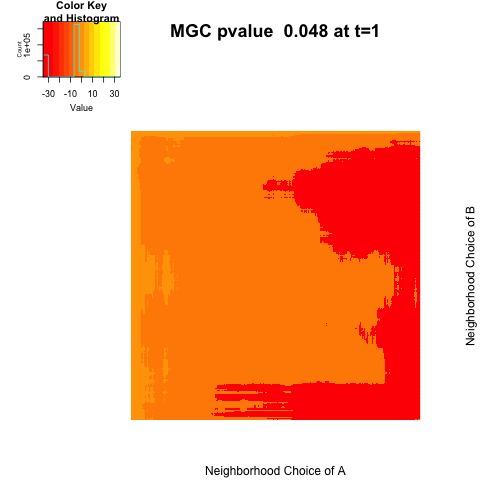
\includegraphics[width=0.4\textwidth]{../figure/pAll21.png}}
\subfigure[t=2]{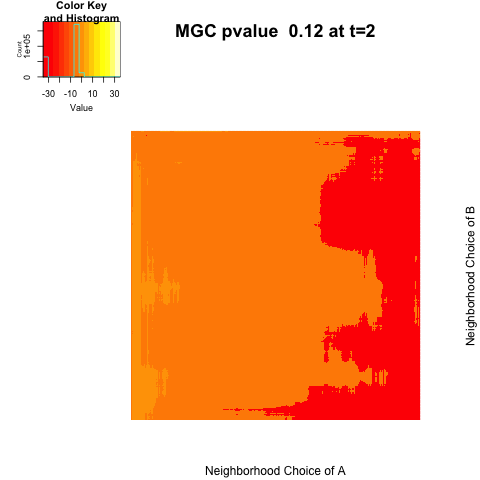
\includegraphics[width=0.4\textwidth]{../figure/pAll22.png}}
\subfigure[t=5]{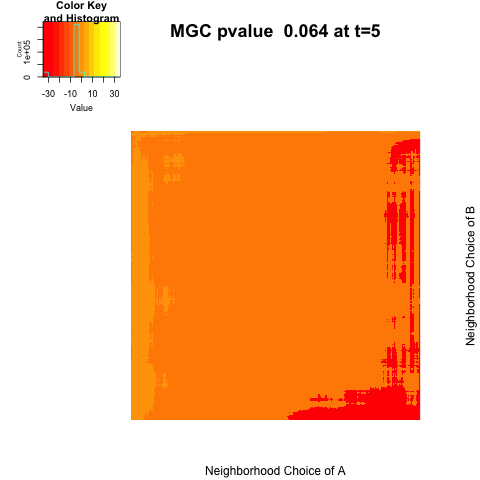
\includegraphics[width=0.4\textwidth]{../figure/pAll25.png}}
\subfigure[t=10]{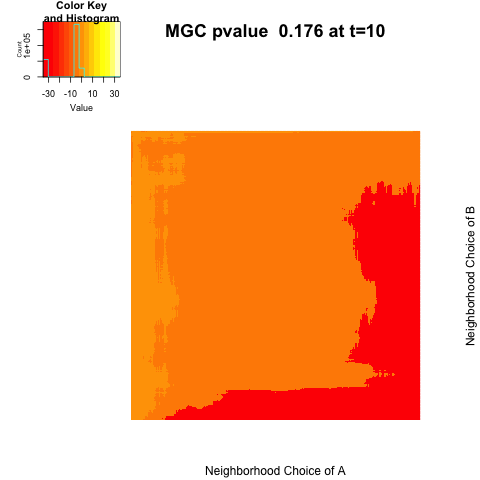
\includegraphics[width=0.4\textwidth]{../figure/pAll210.png}}
\caption{log-scale of P-values when $\rho$ = 0.2}
\label{fig:pAll2}    
\end{figure} 

On the other hand, p-values might \textit{happen to be low} because they are also random variables. Moreover we never know the optimal scale nor power. The following results are from re-sampling procedures. Generate $M=500$ random graphs and their nodes' (1) univariate / (2) multivariate attributes from the same joint distribution. The power of independence is calculated in the following ways:

$$\mbox{Power } = \hat{P}(\mbox{ p-values } \leq 0.05)$$

Before using local test, first test independence via global test using \verb!dcov.test! from \verb!energy! package for \verb!R!. The following table shows the estimated power at different diffusion time points for each correlation coefficient. 


\begin{table}[ht]
\centering
\begin{tabular}{rrrrr}
  \hline
 & t=1 & t=2 & t=5 & t=10 \\ 
  \hline
$\rho$=0.0 & 0.05 & 0.06 & 0.06 & 0.07 \\ 
$\rho$=0.1 & 0.09 & 0.24 & 0.39 & 0.42 \\ 
$\rho$=0.2 & 0.29 & 0.83 & 0.95 & 0.97 \\ 
   \hline
\end{tabular}
\caption{Estimated power based on dCor statistics}
\label{tab:dcor}
\end{table}


\begin{table}[ht]
\centering
\begin{tabular}{rrrrr}
  \hline
 & t=1 & t=2 & t=5 & t=10 \\ 
  \hline
r=0.0 & 0.08 & 0.09 & 0.09 & 0.09 \\ 
  r=0.1 & 0.43 & 0.52 & 0.57 & 0.58 \\ 
  r=0.2 & 0.97 & 0.99 & 0.99 & 1.00 \\ 
   \hline
\end{tabular}
\caption{Estimated power of optimal local tests}
\label{tab:local}
\end{table}


Table \ref{tab:dcor} illustrates changing (estimated) power as time goes. It is noticeble that the estimated power increases as diffusion process continues. Table \ref{tab:local} shows the estimated power at local optimal scale, where reaches the highest power. The area of reaching highest power as well as estimated power at local scale is increasing as the time point $t$ increases under $H_{A}.$ 


%%%%%%%%%%%%%%%%%%% power heatmap %%%%%%%%%%%%%%%%%%%%

\begin{figure}[H]
\captionsetup{format=plain}
\centering
\subfigure[t=1]{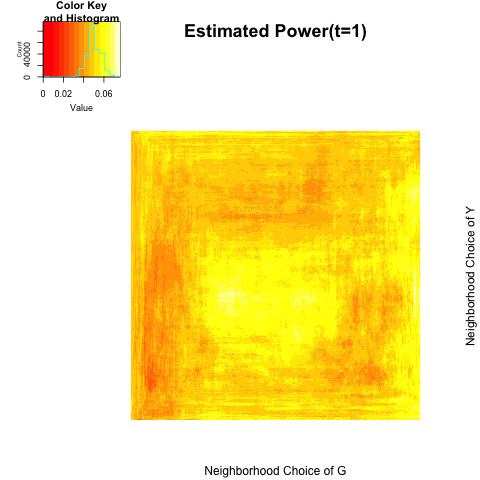
\includegraphics[width=0.4\textwidth]{../figure/power0_1.png}}
\subfigure[t=2]{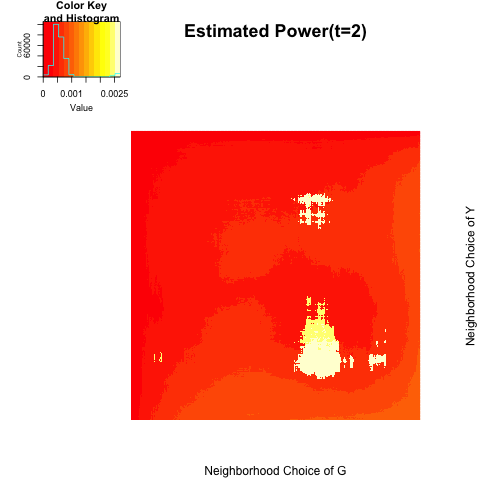
\includegraphics[width=0.4\textwidth]{../figure/power0_2.png}}
\subfigure[t=5]{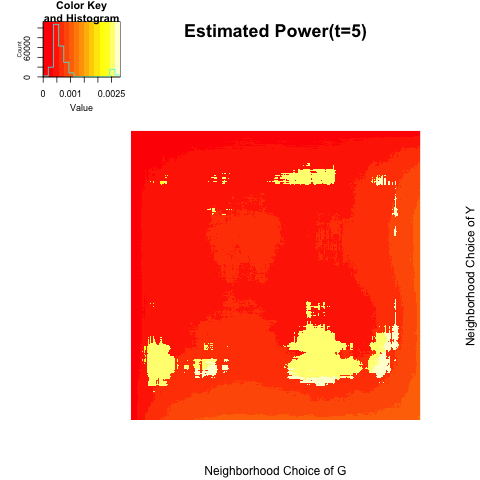
\includegraphics[width=0.4\textwidth]{../figure/power0_5.png}}
\subfigure[t=10]{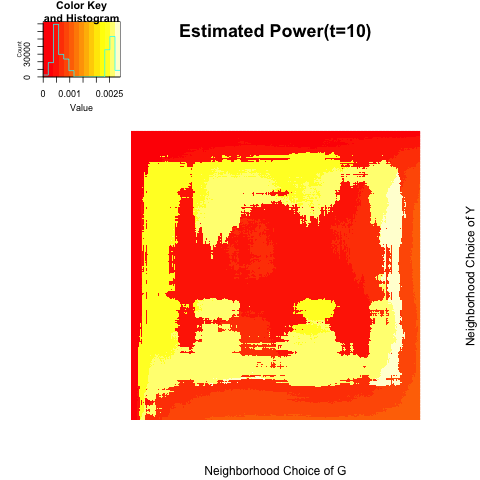
\includegraphics[width=0.4\textwidth]{../figure/power0_10.png}}
\caption{Estimated power when $\rho$ = 0.0}
\label{fig:power0}    
\end{figure} 


\begin{figure}[H]
\captionsetup{format=plain}
\centering
\subfigure[t=1]{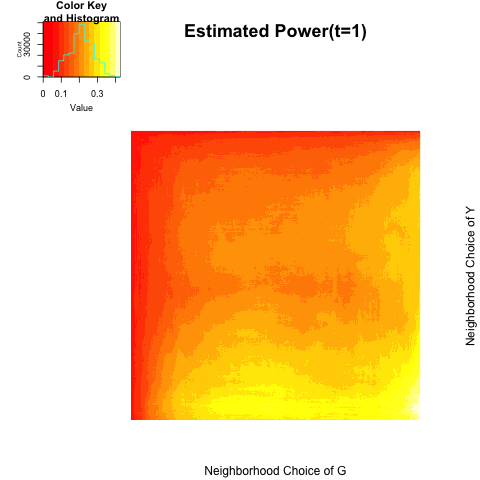
\includegraphics[width=0.4\textwidth]{../figure/power1_1.png}}
\subfigure[t=2]{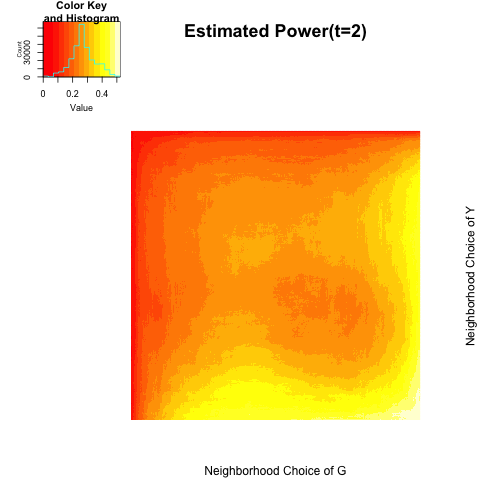
\includegraphics[width=0.4\textwidth]{../figure/power1_2.png}}
\subfigure[t=5]{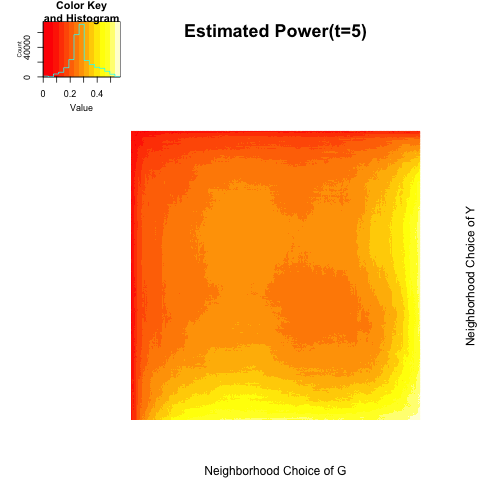
\includegraphics[width=0.4\textwidth]{../figure/power1_5.png}}
\subfigure[t=10]{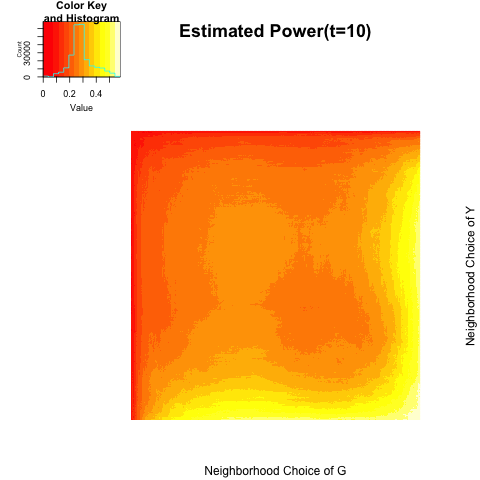
\includegraphics[width=0.4\textwidth]{../figure/power1_10.png}}
\caption{Estimated power when $\rho$ = 0.1}
\label{fig:power1}    
\end{figure} 
 
 
 
\begin{figure}[H]
\captionsetup{format=plain}
\centering
\subfigure[t=1]{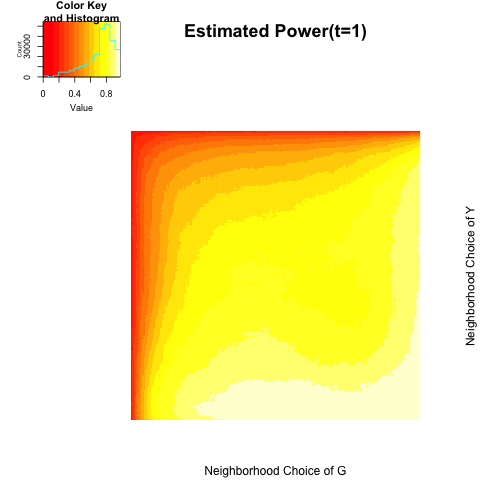
\includegraphics[width=0.4\textwidth]{../figure/power2_1.png}}
\subfigure[t=2]{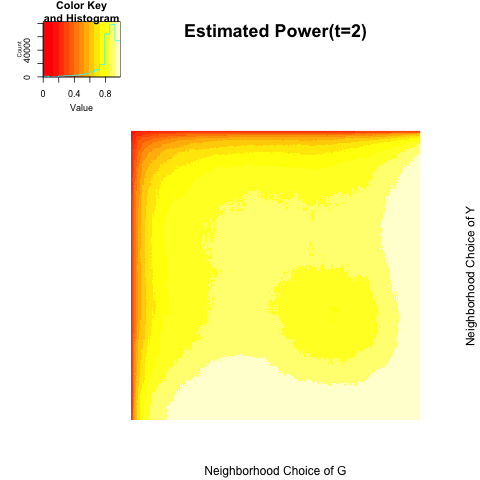
\includegraphics[width=0.4\textwidth]{../figure/power2_2.png}}
\subfigure[t=5]{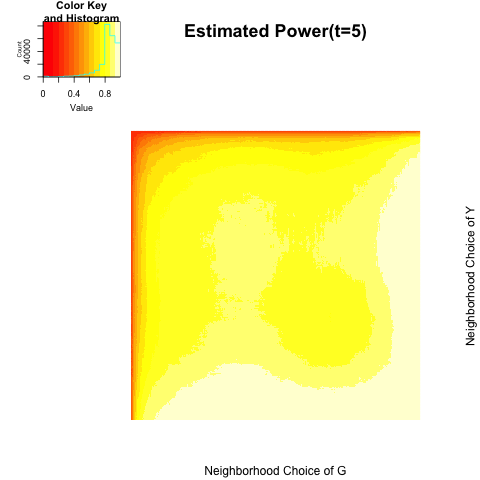
\includegraphics[width=0.4\textwidth]{../figure/power2_5.png}}
\subfigure[t=10]{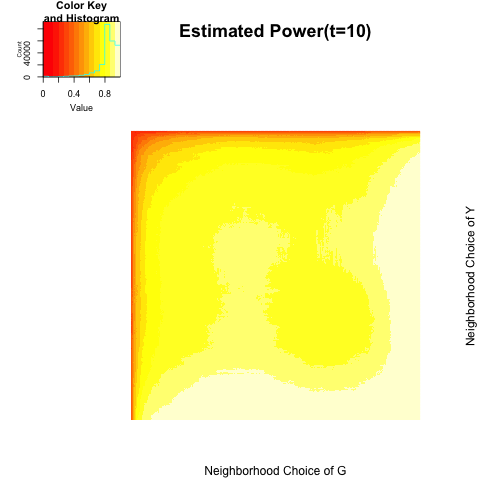
\includegraphics[width=0.4\textwidth]{../figure/power2_10.png}}
\caption{Estimated power when $\rho$ = 0.2}
\label{fig:power2}    
\end{figure} 
  
 





%%%%%%%%%%%%%%%%%%%%%%%%%%%%%%%%%%%%%%%%%%%%%%%%%%%%%%%%%%%%%%%%%%%%%%%%%
\newpage
\section{Simulation results for univariate case}

\begin{equation} 
\label{eq:latent}
(X_1, Y_{11}, Y_{12}, Y_{13}), ... , (X_N, Y_{1N}, Y_{2N}, Y_{3N})  \overset{i.i.d}{\sim} N \left( \begin{bmatrix} 0 \\ 0 \\ 0 \\ 0 \end{bmatrix}, \begin{bmatrix}1 & \rho_{1} & \rho_{2}&  \rho_{3} \\ \rho_{1} & 1 & 0 & 0 \\ \rho_{2} & 0 & 1 & 0 \\ \rho_{3} & 0 & 0 & 1  \end{bmatrix}  \right)
\end{equation}

\textbf{(0) $\rho = (\rho_{1}, \rho_{2}, \rho_{3}) = (0.0, 0.0, 0.0)$}

%%%%%%%%%%%%%%%%%%%%%%%%%%%%%%%%%%%%%%%%%%%%%%%%%%%%%%%%%%%%%%%%%%%%%%%%%
\newpage
\textbf{(1) $\rho = (\rho_{1}, \rho_{2}, \rho_{3}) = (0.1, 0.1, 0.1)$}

\begin{figure}[H]
\captionsetup{format=plain}
\centering
\subfigure[t=1]{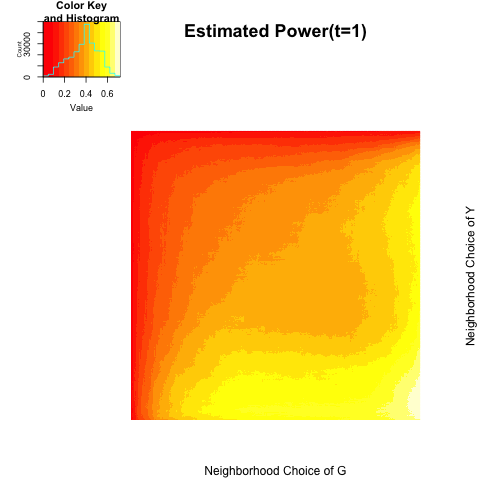
\includegraphics[width=0.4\textwidth]{../figure/multi1_1.png}}
\subfigure[t=2]{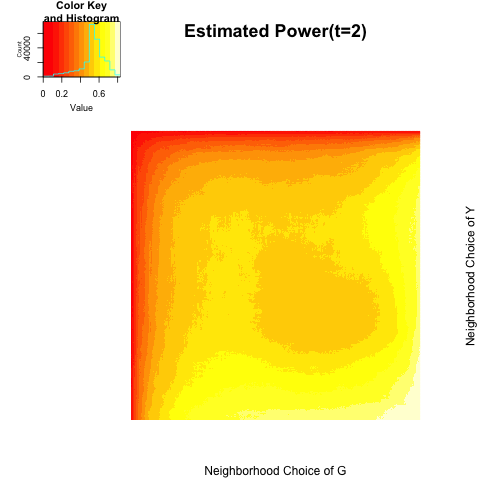
\includegraphics[width=0.4\textwidth]{../figure/multi1_2.png}}
\subfigure[t=5]{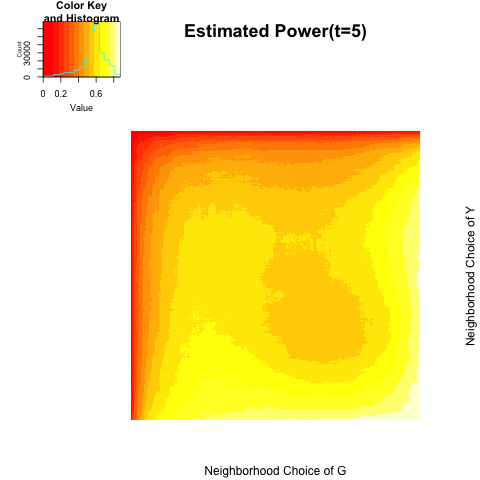
\includegraphics[width=0.4\textwidth]{../figure/multi1_5.png}}
\subfigure[t=10]{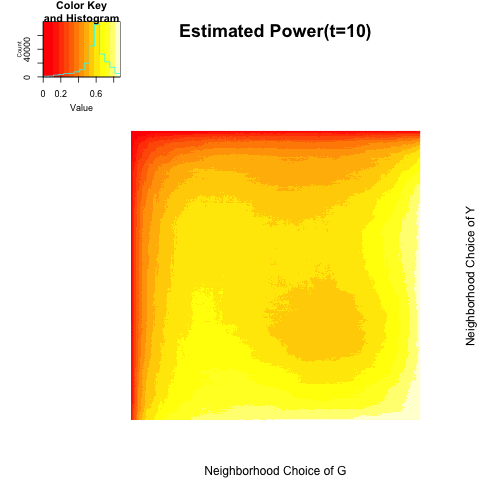
\includegraphics[width=0.4\textwidth]{../figure/multi1_10.png}}
\caption{Estimated power when $\rho$ = (0.1, 0.1, 0.1)}
\label{fig:multi1}    
\end{figure} 
 
\begin{table}[ht]
\centering
\begin{tabular}{rrrrr}
  \hline
 & t=1 & t=2 & t=5 & t=10 \\ 
  \hline
global test & 0.12 & 0.41 & 0.65 & 0.69 \\ 
  local optimal & 0.72 & 0.83 & 0.87 & 0.87 \\ 
   \hline
\end{tabular}
\caption{Estimated power of multivariate attribute model 1}
\end{table}




%%%%%%%%%%%%%%%%%%%%%%%%%%%%%%%%%%%%%%%%%%%%%%%%%%%%%%%%%%%%%%%%%%%%%%%%%%
\newpage
\textbf{(2) $\rho = (\rho_{1}, \rho_{2}, \rho_{3}) = (0.2, 0.2, 0.2)$}


\begin{figure}[H]
\captionsetup{format=plain}
\centering
\subfigure[t=1]{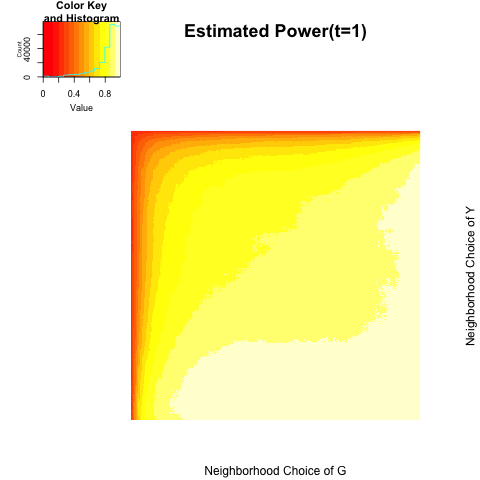
\includegraphics[width=0.4\textwidth]{../figure/multi2_1.png}}
\subfigure[t=2]{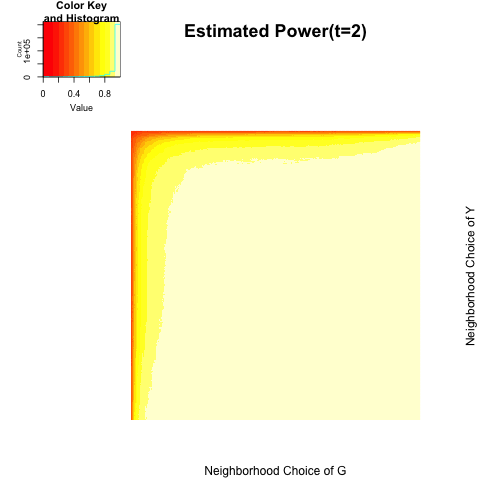
\includegraphics[width=0.4\textwidth]{../figure/multi2_2.png}}
\subfigure[t=5]{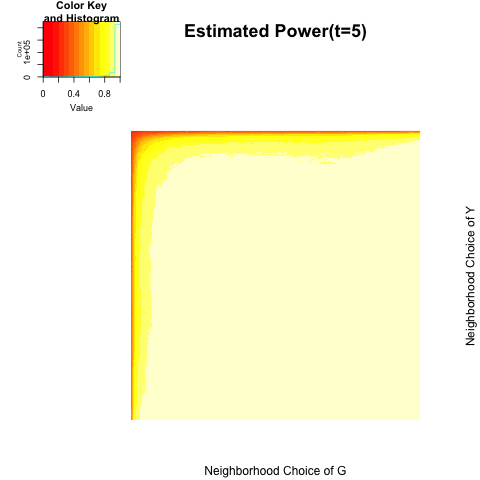
\includegraphics[width=0.4\textwidth]{../figure/multi2_5.png}}
\subfigure[t=10]{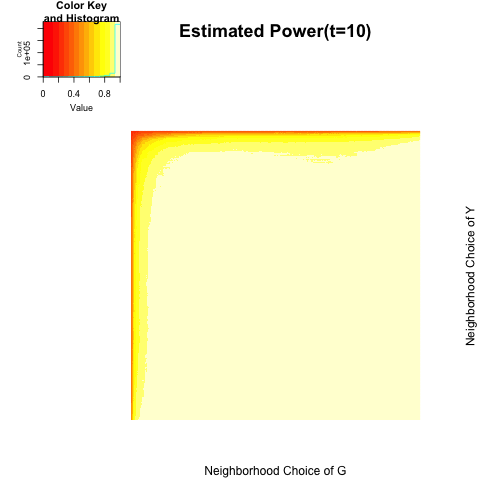
\includegraphics[width=0.4\textwidth]{../figure/multi2_10.png}}
\caption{Estimated power when $\rho$ = (0.2, 0.2, 0.2)}
\label{fig:multi2}    
\end{figure} 


\begin{table}[ht]
\centering
\begin{tabular}{rrrrr}
  \hline
 & t=1 & t=2 & t=5 & t=10 \\ 
  \hline
global test & 0.64 & 1.00 & 1.00 & 1.00 \\ 
  local optimal & 0.99 & 1.00 & 1.00 & 1.00 \\ 
   \hline
\end{tabular}
\caption{Estimated power of multivariate attribute model 2}
\end{table}

%%%%%%%%%%%%%%%%%%%%%%%%%%%%%%%%%%%%%%%%%%%%%%%%%%%%%%%%%%%%%%%%%%%%%%%%%%
%\newpage
\textbf{(3) $\rho = (\rho_{1}, \rho_{2}, \rho_{3}) = (0.2, 0.0, 0.0)$}

%%%%%%%%%%%%%%%%%%%%%%%%%%%%%%%%%%%%%%%%%%%%%%%%%%%%%%%%%%%%%%%%%%%%%%%%%
%\newpage
\textbf{(4) $\rho = (\rho_{1}, \rho_{2}, \rho_{3}) = (0.2, 0.2, 0.0)$}

%%%%%%%%%%%%%%%%%%%%%%%%%%%%%%%%%%%%%%%%%%%%%%%%%%%%%%%%%%%%%%%%%%%%
\newpage
\textbf{(5) $\rho = (\rho_{1}, \rho_{2}, \rho_{3}) = (0.2, -0.2, 0.0)$}


\begin{figure}[H]
\captionsetup{format=plain}
\centering
\subfigure[t=1]{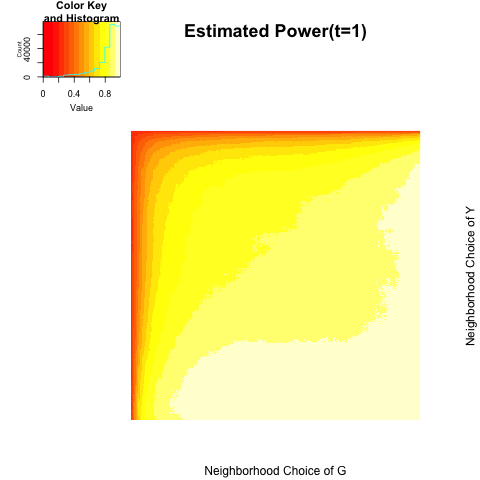
\includegraphics[width=0.4\textwidth]{../figure/multi5_1.png}}
\subfigure[t=2]{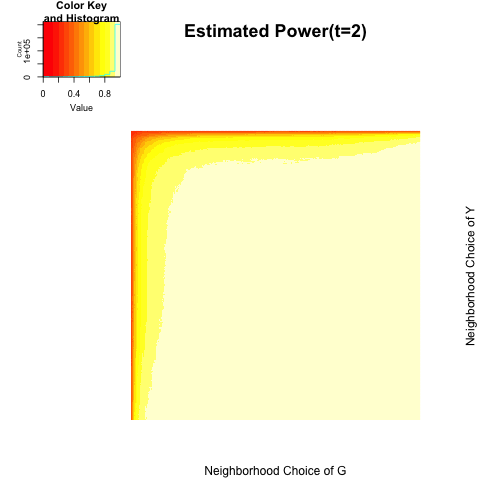
\includegraphics[width=0.4\textwidth]{../figure/multi5_2.png}}
\subfigure[t=5]{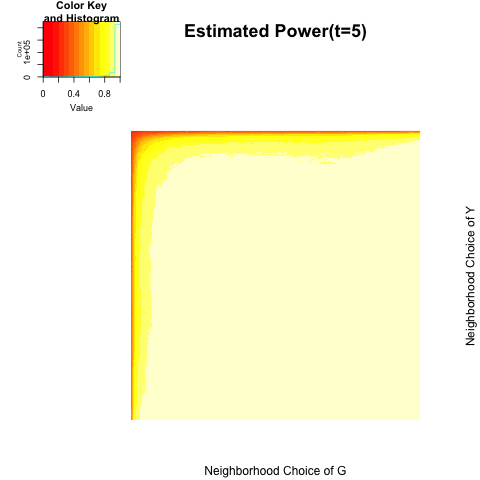
\includegraphics[width=0.4\textwidth]{../figure/multi5_5.png}}
\subfigure[t=10]{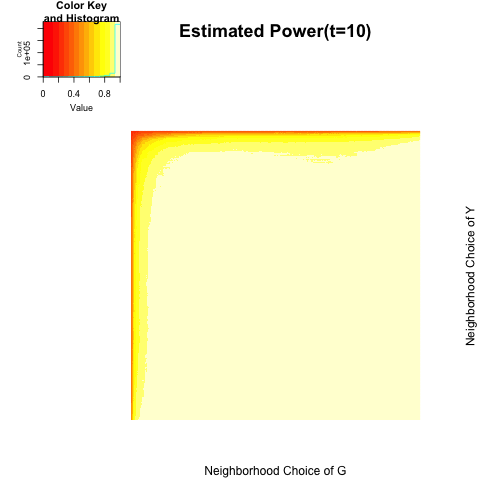
\includegraphics[width=0.4\textwidth]{../figure/multi5_10.png}}
\caption{Estimated power when $\rho$ = (0.2, -0.2, 0.0)}
\label{fig:multi5}    
\end{figure} 
 

\begin{table}[ht]
\centering
\begin{tabular}{rrrrr}
  \hline
 & t=1 & t=2 & t=5 & t=10 \\ 
  \hline
global test & 0.40 & 0.91 & 0.99 & 0.99 \\ 
  local optimal & 0.99 & 1.00 & 1.00 & 1.00 \\ 
   \hline
\end{tabular}
\caption{Estimated power of multivariate attribute model 5}
\end{table}


\newpage
\section{Test independence between two graphs(networks)}

\subsection{Dependent Latent Variable Model}

Assume a network $H$ and $G$ have same node index - maybe they are all considering same individuals but different networks. Someone might be interested in independence between online friendship and offline friendship; independence between physical connections and functional relationship, etc. 

$$H_{0}: f_{GH}  = f_{G} f_{H}$$

For all nodes $i \neq j$ in a graph $G$, and all nodes $u \neq v$ in a graph $H$, suppose the following latent variable model:

\begin{equation} 
\label{eq:latent}
(X_1, W_1), (X_2, W_2) , ... , (X_N, W_N)  \overset{i.i.d}{\sim} N \left( \begin{bmatrix} 0 \\ 0 \end{bmatrix}, \begin{bmatrix}1 & \rho \\ \rho & 1 \end{bmatrix}  \right)
\end{equation}


\begin{equation}
\label{eq:latentspace}
\log \left( \frac{P\big( T_{ij} \big) }{1 - P\big( T_{ij}    \big) } \big| X_i, X_j \right) = f \big( | X_i - X_j |  \big) = \log \left( \frac{P\big( T_{uv} \big) }{1 - P\big( T_{uv}    \big) } \big|W_i, W_j   \right)
\end{equation}

\newpage
\textbf{Simulation Result}


(1) $\rho = 0.0$ ($M = 500$ iterations; $n = 300$)

\begin{figure}[H]
\captionsetup{format=plain}
\centering
\subfigure[t=1]{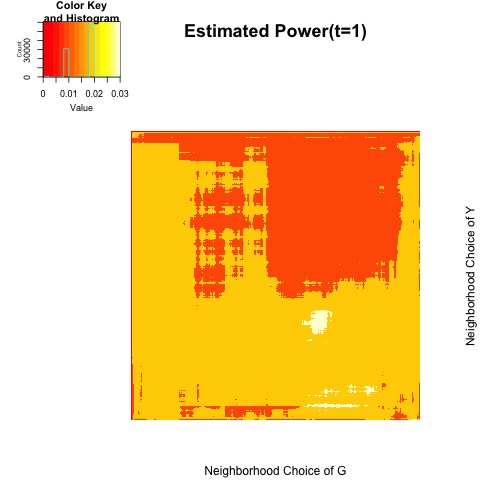
\includegraphics[width=0.4\textwidth]{../figure/gh1_1.png}}
\subfigure[t=2]{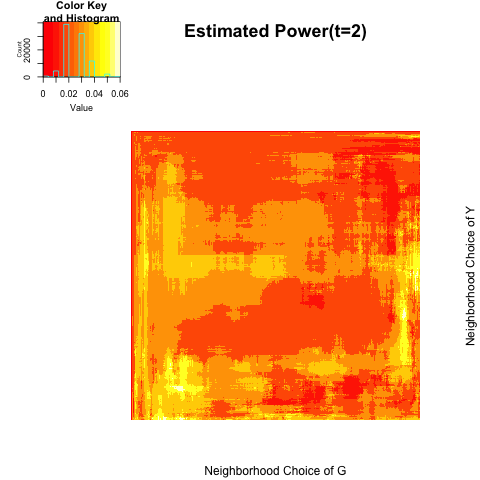
\includegraphics[width=0.4\textwidth]{../figure/gh1_2.png}}
\subfigure[t=5]{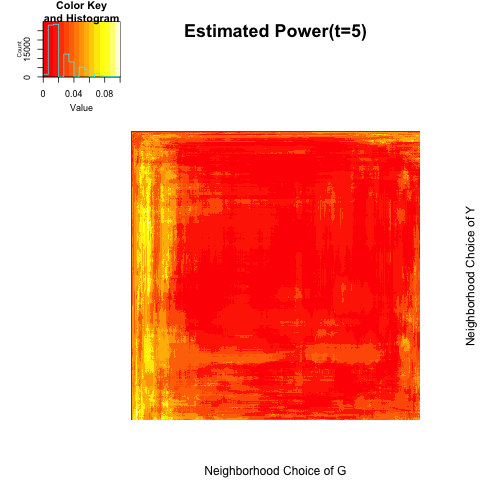
\includegraphics[width=0.4\textwidth]{../figure/gh1_5.png}}
\subfigure[t=10]{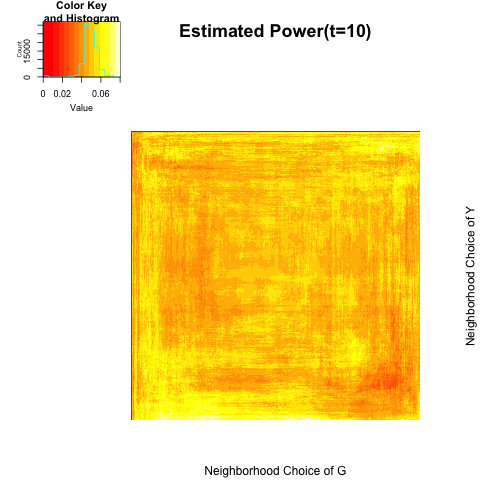
\includegraphics[width=0.4\textwidth]{../figure/gh1_10.png}}
\caption{Estimated power when $\rho$ = 0.0}
\label{fig:gh1}    
\end{figure} 



\begin{table}[ht]
\centering
\begin{tabular}{rrrrr}
  \hline
 & t=1 & t=2 & t=5 & t=10 \\ 
  \hline
global test & 0.05 & 0.06 & 0.06 & 0.05 \\ 
  local optimal & 0.07 & 0.07 & 0.08 & 0.08 \\ 
   \hline
\end{tabular}
\caption{G vs H when $\rho = 0.0$}
\end{table}


\newpage
(2) $\rho = 0.1$ ($M = 500$ iterations; $n = 300$)

\newpage
(3) $\rho = 0.2$ ($M = 500$ iterations; $n = 300$)





%%%%%%%%%%%%%%%%%%%%%%%%%%%%%%%%%%%%%%%%%%%%%%%%%%%%%%%%%%%%%%%%%%%%%%%%%%%%
\newpage
\section{Application to Real Data}

- Similarity measure $\omega$

$$\omega[i,j] = \mbox{ (the number of synapses starting from i to j)}$$
 

- Transition probability (Assume time homogeneous Markov chain; left stochastic matrix)

$$P[i,j] = Pr\big( X_{n} = j  | X_{n-1} = i \big)$$

We define the transition matrix \textbf{P} = $(p_{ij})$ of a Markov chain as:

$$p_{ij} = \left\{ \begin{array}{ll} \frac{w(\{ i, j\})}{ deg(i) } & \mbox{ if } u \sim v \\ 0 & \mbox{ otherwise }  \end{array}  \right.$$


\begin{figure}[H]
\captionsetup{format=plain}
\centering
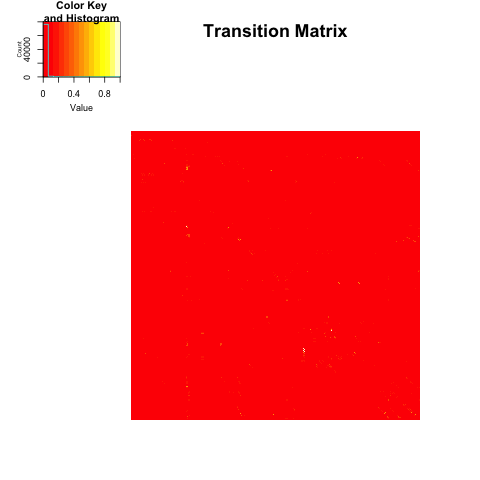
\includegraphics[width=0.4\textwidth]{../figure/trans.png}
\caption{Transition matrix P}
\label{fig:trans}
\end{figure}



- Stationary distribution 
: A probability vector $\pi$ is a stationary distribution for Markov chain $P$ if $\pi P = \pi$. Over the long run, no matter what the starting state was, the proportion of time the chain spends in node $j$ is approximately $\pi(j) (j = 1, ... , n)$.
Use \verb!statdistr! in r.


\begin{figure}[H]
\captionsetup{format=plain}
\centering
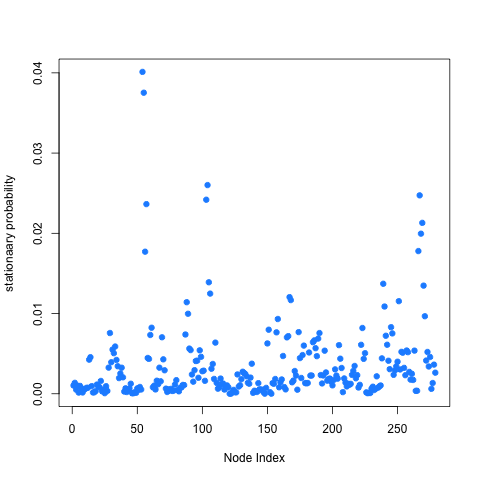
\includegraphics[width=0.4\textwidth]{../figure/statd.png}
\caption{Stationary probability based on P}
\label{fig:statd}
\end{figure}


  Let $G = (V, E, \omega)$ be an undirected graph with $\omega$ being a similarity measure between vertices of $V.$ Denote by $\textbf{P}$ the probability transition matrix of $G.$ The diffusion distance at time $t,$ $\rho_{t}(u,v)$, between two nodes $u,v \in V$ is defined as:
  
  $$\rho^2_{t} = \sum\limits_{w \in V}\big( \textbf{P}^{t}(u,w) - \textbf{P}^{t}(v,w) \big)^2 \frac{1}{\pi(w)} =  \kappa(\textbf{P}^{2t} \Pi^{-1} )$$

 
Diffusion distances for Directed Graph at time $t$ is defined as :

$$\Delta_{\rho^{2}_{t}} = \kappa(\textbf{P}^{t} \Pi^{-1} (\textbf{P}^{t})^{T} )$$
 
where $\kappa(\textbf{A}) = \textbf{A}_{dg} \textbf{1} \textbf{1}^{T} - \textbf{A} - \textbf{A}^{T} + \textbf{1} \textbf{1}^{T} \textbf{A}_{dg}$ 

 
\begin{figure}[H]
\captionsetup{format=plain}
\centering
\subfigure[dissimilarity matrix]{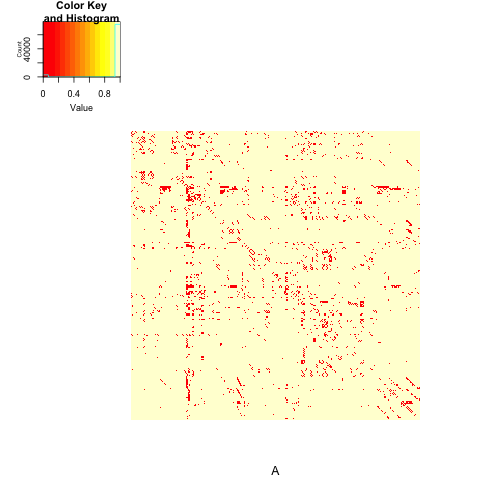
\includegraphics[width=0.3\textwidth]{../figure/A_plot.png}}
\subfigure[t=1]{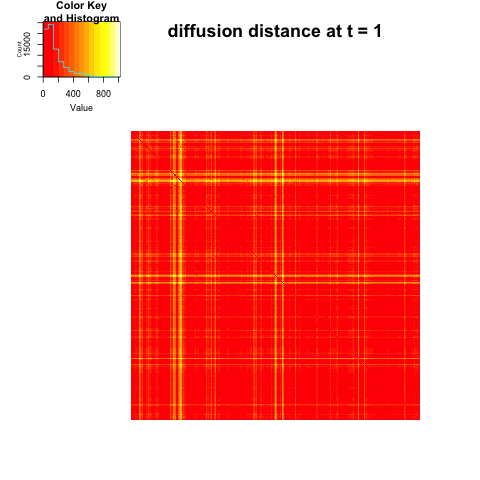
\includegraphics[width=0.3\textwidth]{../figure/diffusion1}}
\subfigure[t=5]{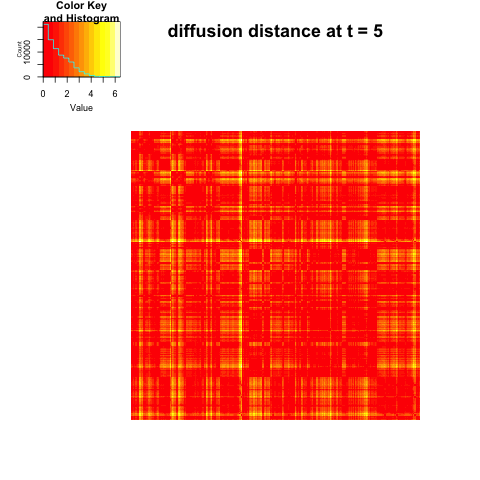
\includegraphics[width=0.3\textwidth]{../figure/diffusion5.png}}
\caption{Heatmap of distance measures}
\label{fig:dist}    
\end{figure} 
 
  
- Difficulties of applying diffusion distance to categorical variable graph : $G$ must be connected. Otherwise, transition probability between different categories will be zero.  

 
\end{document}
